% Faz com que o ínicio do capítulo sempre seja uma página ímpar
\cleardoublepage

% Inclui o cabeçalho definido no meta.tex
\pagestyle{fancy}

% Números das páginas em arábicos
\pagenumbering{arabic}

\chapter{Introdução}\label{intro}

O sistema de controle de atitude e órbita é uma das tecnologias mais críticas de qualquer sistema espacial. O desenvolvimento de um sistema de controle de atitude em território nacional permanece incompleto \citep{Veloso2009} e a venda de componentes deste sistema ao nosso país é frequentemente recusada por países detentores dessa tecnologia.

Basicamente, um sistema de controle de atitude é formado por sensores, atuadores e uma central responsável pelo processamento dos sinais dos sensores e comando dos atuadores, segundo uma lei de controle. Os sensores mais comuns são detectores de horizonte, sensores magnéticos, sensores solares, giroscópios e rastreadores estelares. 

Os principais atuadores incluem: propulsores, torques magnéticos e rodas de reação. A quase totalidade destes componentes de controle possui atualmente alguma iniciativa de desenvolvimento no país, seja por instituições governamentais ou por grupos de pesquisa independentes \citep{PresidenciaRepublica}. A principal exceção são as rodas de reação, que praticamente não têm projetos de desenvolvimento em andamento e, no entanto, representam um componente indispensável na realização de manobras e na estabilização e controle de atitude em três eixos. 

Rodas de reação são dificilmente substituíveis pois apresentam larga faixa de operação em torque (ao contrário de atuadores magnéticos) e são alimentadas pela energia renovável fornecida por painéis solares (ao contrário de propulsores baseados em um estoque finito de combustível). Por estes motivos, rodas de reação estão presentes em praticamente qualquer satélite que apresente requerimentos mínimos de desempenho em atitude.

Uma roda de reação pode ser descrita como um atuador inercial com funcionamento baseado no princípio de conservação do momento angular. A atuação da roda de reação sobre o satélite se realiza por intercâmbio de momento angular, limitado ao eixo de rotação da roda. Devido a grande diferença entre a inercia do satélite e o da roda de reação, um controle de atitude com muita precisão é possível com esse sistema.

Rodas de reação são tipicamente constituídas de um motor elétrico, geralmente um motor sem escovas, um mancal e um elemento de inércia.  O elemento de inércia e o motor são montados sobre o mancal que deve garantir a  precisa rotação em torno de um eixo. A velocidade de rotação do sistema é controlado por uma eletrônica de acionamento do motor. Rodas de reação podem ser comandada de duas maneiras distinta: por rotação ou por torque. Quando comandada por torque, a roda de reação deve ser capaz de estimar o torque útil gerado por ela (o torque efetivo menos as perdas). 

O controle de atitude  com rodas de reação demanda que esse tipo de  atuador opere em toda sua escala de velocidade, inclusive na inversão de seu sentido de rotação (passagem pelo zero) de uma forma estável e controlada. Essa zona morta é efeito do atrito estático do mancal, minimizar esse efeito é essencial para o bom funcionamento da roda de reação. A zona morta pode ser compensada (no caso de mancal por rolamento) pela implementação de leis de controle com malhas de velocidade e corrente, além de um estimador de atrito.

O projeto de uma roda de reação começa pelo estudo do momento angular necessário para movimentar o satélite, com o momento angular definido especifica-se a inércia e então o mancal, por último projeta-se um motor capaz de rotacionar o conjunto mancal mais inércia.


\section{Objetivo}

Essa dissertação vem ao encontro de projetar um mancal magnético para uma roda de reação que está sendo desenvolvido no Núcleo de Sistemas Eletrônicos Embarcados (NSEE) do Instituto Mauá De Tecnologia (IMT) com apoio do Instituto Nacional De Pesquisas Espaciais (INPE).

O projeto envolve o desenvolvimento de um conjunto eletromecânico capaz de ser utilizado em uma roda de reação para satélites de médio porte mais especificamente para a plataforma multi missão.

%\todo[color=magenta]{Ref. Roda de Reacão - Mauá}

\section{Justificativa}

A suspensão do rotor com relação ao estator representa uma parte crítica em rodas de reação \citep{taniwaki2003experimental} devido as consequências de qualquer fricção no movimento relativo entre estes dois componentes. Com efeito, a fricção se traduz não apenas em um maior consumo de potência elétrica, como também na introdução de uma zona morta de atuação em torque, bem como na limitação da vida útil da roda de reação devido ao gradual desgaste do mancal.

Uma solução mecânica para a interface entre o rotor e o estator é o mancal por rolamento. Apesar de sua aparente simplicidade, apresenta desafios para a obtenção dos valores mínimos de fricção necessários, em vista das exigências de consumo, controlabilidade e vida útil da roda de reação \citep{Krishnan2010}. No caso de aplicações aerospaciais, a lubrificação do rolamento representa também considerável dificuldade devido à impossibilidade de utilização de lubrificantes tradicionais em condições de baixa ou nenhuma pressão atmosférica, que leva à perda dos componentes voláteis destes lubrificantes e sua consequente degradação. Outra dificuldade se deve à tendência de migração dos lubrificantes na ausência de gravidade, o que costuma ser abordado com estratégias de recaptura ou relubrificação. Sistemas de relubrificação, em particular, apresentam grande complexidade e seu comportamento orbital é de difícil validação em laboratório.

As dificuldades associadas ao uso de mancal de rolamento reside também em sua modelagem, consequência da variação de viscosidade do lubrificante em função da temperatura do mancal, o que torna o coeficiente de fricção dependente da velocidade de rotação e das condições térmicas em geral. O mancal por rolamento apresenta, por outro lado, grande vantagem construtiva devido a compactação do sistema e não necessidade de eletrônica extra para o seu controle. 

Outra solução é a utilização de um mancal magnético \citep{Bangcheng2012},  que é uma alternativa sem contato mecânico entre o rotor e o estator, na qual o rotor é mantido suspenso magneticamente. O ganho em confiabilidade e vida útil da roda de reação é considerável \citep{Marble2006}, sendo a vida útil basicamente limitada  pela durabilidade da eletrônica. A operação sem contato elimina a necessidade de lubrificante e possibilita consequentemente a operação em vácuo, o que se traduz em simplificação nos requisitos da concepção mecânica. 

A ausência de fricção elimina a zona morta de aplicação de torque em baixas velocidades, eliminando não-linearidades da lei de controle, além de possibilitar a eliminação de defeitos de balanceamento e vibrações mecânicas, com consequente ganho em simplicidade dos algoritmos e em desempenho do controle de atitude. A contrapartida é a adição de uma malha de controle para a suspensão eletromagnética. O ganho de eficiência trazido pela ausência de fricção também é contrabalanceado, ao menos parcialmente, pelo consumo de potência dos atuadores deste tipo de mancal.

\section{Revisão bibliográfica}

%\begin{footnotesize}
%\textbf{Conteúdo:}
%\begin{enumerate}
%	\item Historia do Mancal Magnético
%	\item Falar de que não pode existir uma mancal puramente passivo (Earnshaw's theorem)
%	\item Tipos de MM (graus de liberdade)
%	\item Utilização do MM.
%	\item Detalhar uso em satélites (exaltar problemas)
%	\item Técnicas de controle aplicadas em MM.
%\end{enumerate}
%\end{footnotesize}

%Estudo iniciais sobre mancais magnéticos são datados do seculo XIX \citep{Weise1989} porem só recentemente começaram a ter grandes aplicados na sociedade, os primeiros mancais magnéticos alguns exemplos são : equipamentos médicos, corações artificiais, bombas de vácuo, motores de altas rotações. Mancais magnéticos fazem uso extensivo de campos magnéticos e tiveram uma grande evolução quando os imãs de terras raras tornaram-se cada vez mais comerciais, aumentando a capacidade de geração de campos permanentes.


%A suspensão do rotor com relação ao estator representa uma parte crítica em rodas de reação \citep{taniwaki2003experimental} devido as consequências de qualquer fricção no movimento relativo entre estes dois componentes. Com efeito, a fricção se traduz não apenas em um maior consumo de potência elétrica, como também na introdução de uma zona morta de atuação em torque, bem como na limitação da vida útil da roda de reação devido ao gradual desgaste do mancal. 
%
%Uma solução mecânica para a interface entre o rotor e o estator é o mancal por rolamento. Apesar de sua aparente simplicidade, apresenta desafios para a obtenção dos valores mínimos de fricção necessários, em vista das exigências de consumo, controlabilidade e vida útil da roda de reação \citep{Krishnan2010}. No caso de aplicações aerospaciais, a lubrificação do rolamento representa também considerável dificuldade devido à impossibilidade de utilização de lubrificantes tradicionais em condições de baixa ou nenhuma pressão atmosférica, que leva à perda dos componentes voláteis destes lubrificantes e sua consequente degradação. Outra dificuldade se deve à tendência de migração dos lubrificantes na ausência de gravidade, o que costuma ser abordado com estratégias de recaptura ou relubrificação. Sistemas de relubrificação, em particular, apresentam grande complexidade e seu comportamento orbital é de difícil validação em laboratório.



Para contornar os problemas de lubrificação em baixa pressão, algumas rodas de reação  utilizam um sistema hermeticamente selado pressurizado com um gás inerte \citep{Krishnan2010}. Esta solução relaxa os requisitos de lubrificação porém impõe uma força de arrasto extra na roda, restando ainda o problema da migração dos lubrificantes na ausência de gravidade. Uma pesquisa detalhada dos lubrificantes de classe espacial e estratégias de selamento e relubrificação deve ser realizada.

%A outra solução é a utilização de um mancal magnético \citep{Marble2006, Bangcheng2010} que é uma alternativa sem contato mecânico entre o rotor e o estator, na qual o rotor é mantido suspenso magneticamente. O ganho em confiabilidade e vida útil da roda de reação é considerável \citep{Ludner1995}, sendo a vida útil basicamente limitada  pela durabilidade da eletrônica. A operação sem contato elimina a necessidade de lubrificante e possibilita consequentemente a operação em vácuo, o que se traduz em simplificação nos requisitos da concepção mecânica. A ausência de fricção elimina a zona morta de aplicação de torque em baixas velocidades, eliminando não-linearidades da lei de controle, com consequente ganho em simplicidade dos algoritmos e em desempenho do controle de atitude. A contrapartida é a adição de uma malha de controle para a suspensão eletromagnética. O ganho de eficiência trazido pela ausência de fricção também é contrabalanceado, ao menos parcialmente, pelo consumo de potência dos atuadores deste tipo de mancal.
	
Devido as não linearidades do mancal magnético (por exemplo sua rigidez em função do deslocamento), a modelagem analítica é de difícil obtenção e uma análise por elementos finitos é recomendada \citep{pilat2007automatic}. Com este tipo de análise é possível verificar o acoplamento das forças e momentos envolvidos além das características térmicas do sistema. A modelagem e implementação é um terreno fértil para pesquisas em todo o mundo e  esta área ainda é pouco explorada no país. Com a presente pesquisa, pretende-se contribuir com o fechamento da lacuna existente na pesquisa de mancais magnéticos de pequenas dimensões.

\subsection{Graus de liberdade}

Mancais magnéticos puramente passivos são impossíveis de existirem dado que a parte móvel se torna instável quando submetida a campos magnéticos puramente passivos (Teorema de Earnshaw's), devido essa situação torna-se necessário um controle ativo do campo magnético atuante na parte móvel e por consequência das forças. Os mancais magnéticos podem ser classificados pelo número de graus de liberdade controlados ativamente \citep{Schweitzer2009}:

\begin{enumerate}[a)]
	\item  Mancal passivo:
	
	Este mancal totalmente passivo é formado por um rotor contendo um conjunto de imãs permanentes em disposição de Halbach \citep{Detoni2012}, o que leva potencialização do campo magnético adjacente ao rotor. Um conjunto de enrolamentos passivos no estator é excitado por este campo magnético girante. Na eventualidade de qualquer deslocamento do rotor, este enrolamento reage com a criação de um campo magnético, com a consequente atração/repulsão do rotor de volta à posição de equilíbrio. O sistema é estável a partir de uma velocidade de rotação mínima do rotor (velocidade crítica). O fato desta topologia não funcionar em baixas velocidades angulares a torna pouco adaptada para aplicação em rodas de reação.
	
	\item  Mancal ativo num grau de liberdade
	
	Neste caso o rotor e o estator são formados por ímãs permanentes em configuração repulsiva, tornando o sistema estável axialmente. O eixo radial é instável e necessita controle ativo, normalmente realizado por meio de eletro-ímãs. Trata-se de uma configuração necessitando uma eletrônica de controle relativamente simples e de baixo consumo de potência. No entanto, a ausência de controle ativo radial tende a gerar oscilações mecânicas de difícil amortecimento.
	
	\item Mancal ativo em dois graus de liberdade
	
	Neste caso o rotor e o estator compõem um circuito magnético em configuração atrativa, em geral com ímãs permanentes no rotor acoplado a um circuito magnético de baixa relutância no estator. O sistema é estável axialmente mas necessita controle ativo nos dois eixos radiais. Esta configuração resulta num mancal de boa rigidez radial, com arquitetura simplificada e pequenas dimensões, principalmente na direção axial.
	
	\item Mancal ativo em cinco graus de liberdade
	
	Este mancal totalmente ativo é formado por atuadores eletromagnéticos nas duas direções radiais, na direção axial e nos dois modos de rotação radiais. A sua principal vantagem em aplicações em rodas de reação é a possibilidade de atuação em mais de um eixo de rotação, devido à capacidade de manobra do componente de inércia. Trata-se no entanto de um sistema de controle de grande complexidade, com consequente redução de confiabilidade. 
\end{enumerate}

\subsection{Topologias com aplicação em rodas de reação}

Encontramos na literatura três topologias distintas para utilização de mancais magnéticos em rodas de reação, os mancais propostos para esse tipo de aplicação possuem em sua maioria dois graus de liberdade ativos,  e fazem uso de ímãs permanentes para a geração de campos magnéticos para minimizar o consumo elétrico ativo do sistema. Em seguida analisamos os principais pontos desses mancais.

A topologia proposta por \citet{Bernus1998} trabalha com dois graus de liberdades ativos, com ímãs permanentes no rotor e dois estatores: um interno com bobinas para o controlo do fluxo magnético no rotor (por consequência na direção radial) e outro externo para estabilização axial que também contribui com a rigidez axial. 

Nessa topologia (Fig. \ref{Fig:modelo:frances}), um fluxo magnético contínuo é gerado no rotor por ímãs permanentes ali instalados, as bobinas instaladas no estator interno conseguem gerar campos aditivos e subtrativos no rotor (dependente do sentido da corrente). Se o campo for aditivo, pode-se aumentar a rigidez do eixo axial, caso o campo for subtrativo, consegue-se diminuir sua rigidez, tornando assim mais fácil o deslocamento radial do rotor.

\begin{figure}[!ht]
	\centering
	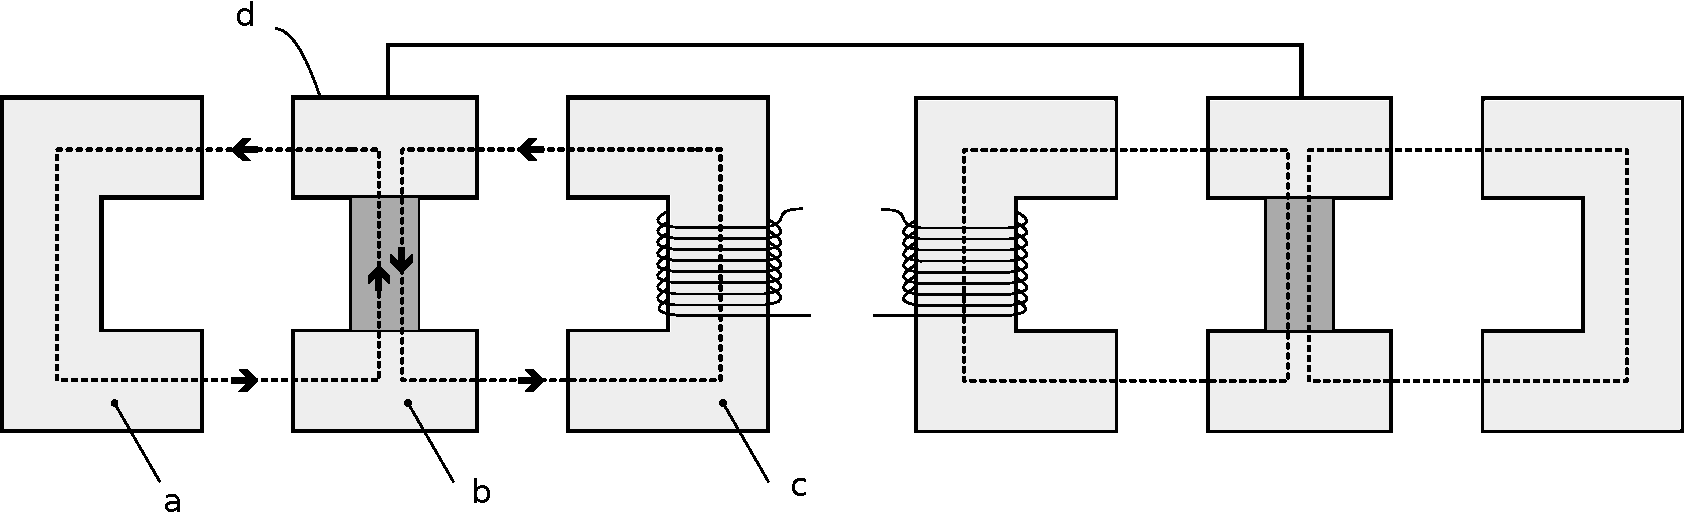
\includegraphics[width=1\linewidth]{./Figs/mancais/frances}
	\caption{Corte da topologia proposta por \cite{Bernus1998} \\
	a: estator externo; b: rotor; c: estator interno; d: ímãs permanentes}
	\label{Fig:modelo:frances}
\end{figure}

A topologia proposta por \citet{Scharfe2001}, difere por ter somente um estator e pelos ímãs permanentes estarem localizados no estator e não no rotor. Como ilustrado na Fig. \ref{Fig:modelo:alemao}. 

%\todo[inline]{falar mais ...}

\begin{figure}[!ht]
	\centering
	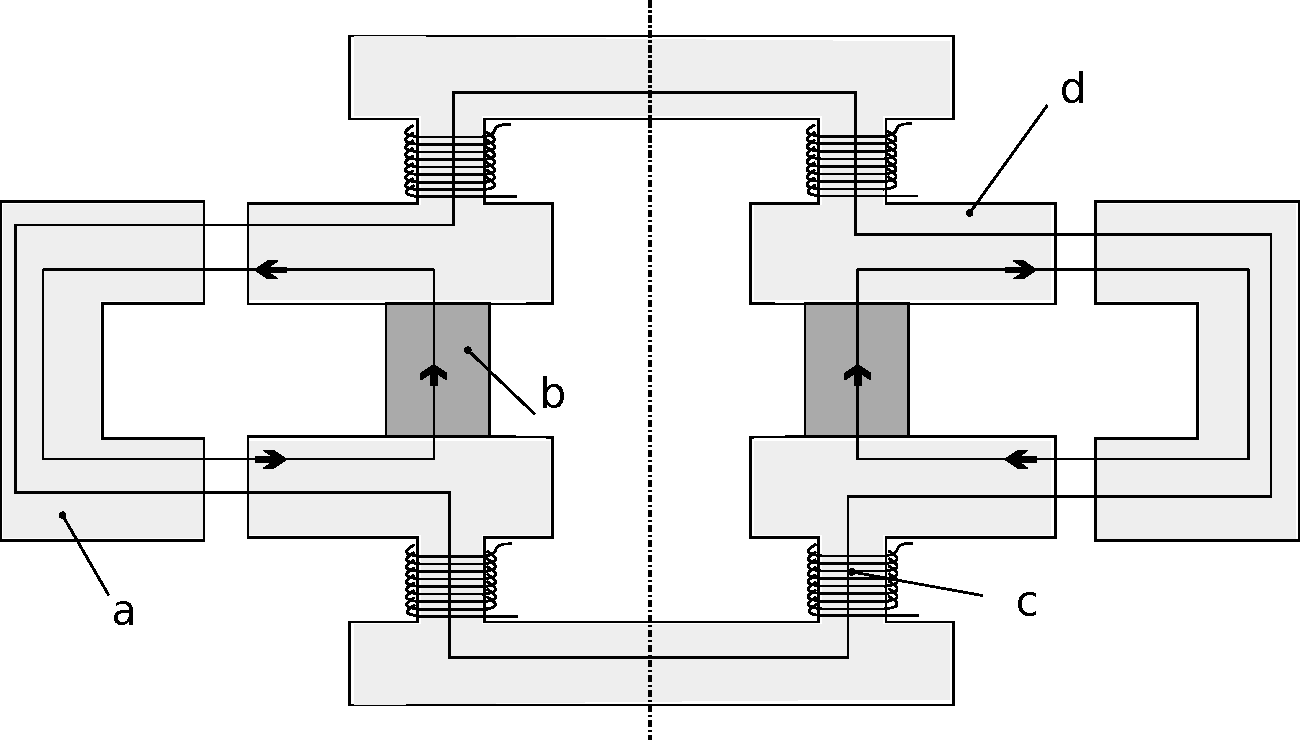
\includegraphics[width=0.8\linewidth]{./Figs/mancais/alemao.pdf}
	\caption{Corte da topologia proposta por \cite{Scharfe2001} \\
	a: estator externo; b: rotor; c: estator interno; d: ímãs permanentes}
	\label{Fig:modelo:alemao}
\end{figure} 

Com essa arquitetura é possível utilizar as bobinas tanto para exercer uma força atrativa no rotor quanto para torna a sua rigidez mas branda, facilitando a atração do rotor. É possível também aumentar a rigidez axial por inserir um fluxo positivo em ambas as bobinas, esse fluxo soma-se com o fluxo do gerado pelos ímãs permanentes.

Mais recentemente uma nova arquitetura foi proposta por \citet{Bangcheng2012} para ser utilizado em uma roda de reação de um satélite ágil.  O rotor é composto de duas partes, uma externa utilizada para estabilizar o mancal na direção axial e outra interna para controle de posição na direção radial. Diferente das outras propostas, essa não utiliza um perfil em C para estabilização dos graus de liberdade passivos, mas sim, faz uso de um perfil plano com ímãs permanentes tanto no rotor quanto no estator.  Ímãs permanentes também usados nos polos do mancal criando um fluxo (\textit{bias}) constante diminuindo a corrente necessária para controlar o rotor.
 
\begin{figure}[!ht]
	\centering
	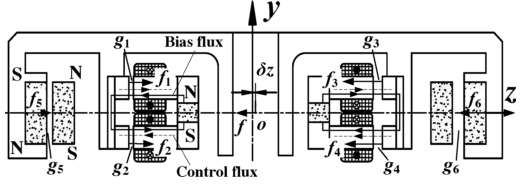
\includegraphics[width=1\linewidth]{./Figs/mancais/chines}
	\caption{Corte da topologia proposta por \cite{Bangcheng2012}}
	\label{Fig:modelo:chines}
\end{figure}

\subsection{Sensoriamento}

 Devido ao controle da posição do rotor em mancais magnéticos, o sensoriamento de sua posição é essencial para o funcionamento do sistema. Duas linhas de sensoriamento são encontradas na literatura: Mancais auto sensoreados \citep{Vischer1993} e os que utilizam sensores de posição dedicados para esse fim.

 Os mancais magnéticos sem sensores (\textit{sensorless}) utilizam geralmente as bobinas de seus polos para sensorear a posição do rotor, diversas técnicas podem ser empregadas \citep{Hofer2009a, Mukhopadhyay2005} entre elas: medição da indutância dos polos pela injeção de um sinal com uma portadora de frequência mais elevada ou a medição da força contra-eletromotriz induzida nas bobinas.
 
 Já os mancais sensoreados utilizam sensores de deslocamentos exclusivos para a medição da posição do rotor e por consequência o tamanho do entreferro. Os sensores podem ser dos tipos capacitivos ou indutivos, dependendo do material construtivo do sistema. Opera-se geralmente com sensores na distribuição diferencial, visando minimizar os efeitos de suas não linearidades.
 
\subsection{Mancais auxiliares}

 Mancais auxiliares são importantes em mancais magnéticos pois são eles que evitam colisões entre as partes fixas e as rotativas em caso de algum tipo de falha, mancais magnéticos projetados para operarem em altas rotações não possuem bom rendimento na inicialização  (baixa rotação) e utilizam dos mancais auxiliares nessa zona até atingirem sua velocidade de operação. Os mancais auxiliares podem ser compostos por rolamentos esféricos \citep{Sun2004a} ou por elementos sólidos auto lubrificante como Teflon.
 
\subsection{Técnicas de controle}

O controle de mancais magnéticos é uma área fértil da engenharia de controle devido as não linearidades do sistema o que torna o projeto do controle não trivial.  

Técnicas de controle clássico são utilizados com bastante frequência em mancais magnéticos, controle do tipo PID  \citep{Tezuka2013} possuem boa robustez. O controle  do tipo \textit{feedforward} é utilizado em casos em que existe o acoplamento entre os graus de liberdade, podendo ser utilizado para o desacoplamento dos graus de liberdade. Outras técnicas propostas na literatura vão de encontro ao controle multivariável como controle robusto \citep{Jimenez-Lizafrraga2007}, controle ótimo (\citep{Schuhmann2012}) e controle não linear (\citep{Rundell1996}).

\section{Metodologia}

A metodologia utilizada no projeto envolve a utilização de simulações em elementos finitos para o projeto das partes magnéticas do mancal, uma modelagem fenomenológica é realizada para o auxilio nas escolhas dos parâmetros físicos do sistema e para o projeto de um simulador.

O desenvolvimento do projeto foi executado como ilustrado na Fig. \ref{fig:metodologia:fluxo:dev}, onde primeiramente as especificações de projeto foram levantadas e uma topologia de mancal proposta com base nos levantamentos bibliográficos.Então foi desenvolvido um modelo em elementos finitos (FEM) e estudos foram realizados em pró de decidir os parâmetros físicos que satisfaçam as restrições emposta para o sistema.

Dividiu-se o projeto em duas partes, na primeiramente considerou-se somente a parte passiva (estator externo e rotor) até atingirmos um conjunto com rigidez suficiente na direção axial e com menor força de atração na direção radial. Com esses valores buscou-se um estator interno capaz de exercer força de atração suficiente no rotor para estabilizar em seu ponto de operação.

%Um protótipo foi construído com base no modelo definido nos passos anteriores e uma avaliação foi feita em busca de 
 
\begin{figure}[th!]
	\centering
	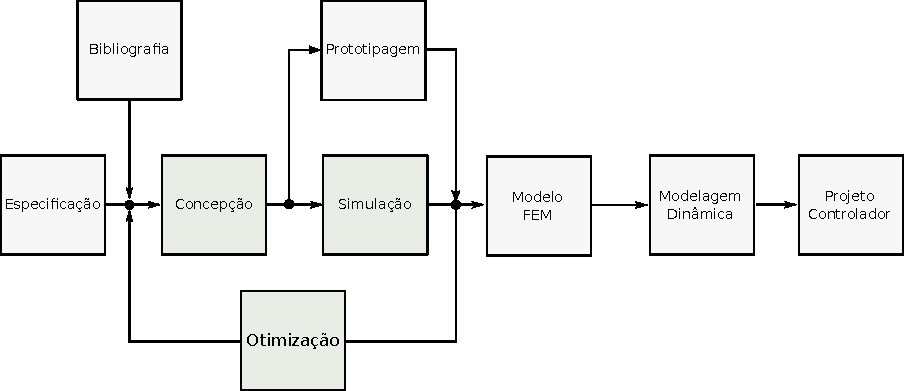
\includegraphics[width=1\linewidth]{Figs/metodologia_fluxo_dev}
	\caption{Fluxo de desenvolvimento}
	\label{fig:metodologia:fluxo:dev}
\end{figure}
 
 
 
% \subsection{Modelagem Elementos Finitos}
% 
%  Foi utilizado como ferramenta de modelagem o Software de elementos finitos e multi física \textit{Comsol}. Nas simulações foram utilizados a curva de histerese do Aço 1020 , as simulações foram realizadas com uma solido tridimensional.  A Fig. \ref{Fig:Simulacao:Passivo:Mesh} ilustra a malha utilizada na execução das simulações com um número aproximado de 19000 elementos.
     
%  	\begin{figure}[!ht]
%  		\centering
%  		\includegraphics[width=0.5 \columnwidth,angle=0]{Figs/Simulacoes/Passivo/3D:Mesh=1,2.png}
%  			\caption{Modelo Comsol do circuito passivo Malha utilizada nos cálculos}
%  			\label{Fig:Simulacao:Passivo:Mesh}
%  	\end{figure}



%\section{Contribuições}

%As contribuições do projeto se estendem para 

%\section{Descrição do conteúdo}


%\todo[inline]{Descrição do documento em geral}